

\section{Reduction through Lifetime}\label{sec:lifetime}
In \autoref{sec:chemlump} is was mentioned that a species lifetime could be used to decide on which species may be lumped together. Here \cite{lifetime} found that large groups of species within the MCM had similar or identical lifetimes and that in many cases this could be attributed to similar/identical rate coefficients for the same type of reaction. This was then used as a methodology for automatic mechanism reduction. 

Using such an approach this section describes a method in which this may be performed without prior knowledge of the mechanism. Natural language processing tools are applied to first determine species of a similar lifetime across a range of timesteps (\autoref{sec:euclid}) and then their standardised temporal profiles are compared (\autoref{sec:cosine}). However, we first begin by defining the lifetime of a species. 

\subsubsection{Calculating the lifetime}
Lifetime is often defined as the time it takes a quantity to halve. In chemical simulations, this translates as the time it would take for a species concentration to decrease by two for a case where the production flux of that species is 0, and all rate constants remain constant. For the first-order decay of sample \autoref{eqn}, we can represent the decay using \autoref{decay}. This shows that the half-life of a species is independent of initial concentration.

\begin{equation}
A \rightarrow[k] B
\label{eqn}
\end{equation}

\begin{equation}
s(t) = a_0 \exp(-kt) \\
\frac{a(t)}{a_0} = \exp(-kt) \\
$$linearised this gives$$
\ln (\frac{a(t)}{a_0}) = -kt
$$ after $\tau_{1/2}$ the concentration is equal to $a_0/2$ of initial rate $a_0$, which gives $$
\ln(\frac{\frac{a_0}{2}}{a_0}) = \ln(\frac{1}{2}) = \ln(2^{-1}) = -\ln2 = k\tau_{1/2}
$$$$
\tau_{\frac{1}{2}} = \frac{\ln 2}{k}
\label{decay}
\end{equation}

In species of the first order only, this may simplified to
\begin{equation}
a(t) = a_0 \exp (t  \sum_j k_j )
$$ and therefore the half life may be written as the reciprocal sum of rate coefficients: $$
\tau_A = 1 / \sum_j k_j
\end{equation}

and is how lifetime is calculated for photochemical species [ref! modelling book, which references pilling and seakings]. An alternative method for half life calculation may be obtained using the diagonal (self reference) of a Jacobian matrix ,\citep{kinetics,lifetime}:

\begin{equation}
\tau_1 = - \frac{1}{J_{ii}}
\end{equation}

This value $J_{ii}$ will usually be negative unless a species does not contain a consuming reaction, then it will be zero.

\subsection{Comparing Magnitude and Direction}
In a simulation the production and loss of species are often directly, or indirectly by other species, influenced by sunlight. This means that the overall production loss fluxes will change with the azimuthal angle of the sun and by consequence the time of the day. As lifetime is calculated using the loss flux of a species, a method that can take temporal changes into account is required to perform lifetime analysis. To do this, a vector containing how a species lifetime changes over the course of a simulation may be obtained from the simulation Jacobians. 

These vectors can then be compared by calculating the euclidean (magnitude) and cosine (angle) distance between pairs of species.  

\subsubsection{Euclidian distance} \label{sec:euclid}
This is the simplest method of vector comparison and works by calculating the distance between all points in two vectors. For the vectors

\begin{equation}
v1 = [ a,b,c, \dots n ]
$$$$
v2 = [ i,j,k, \dots z ]
\end{equation}

This can be done using pythoagoras' theorem in \autoref{euclid}:

\begin{equation}
e_{dist}  = \sqrt{(a-i)^2 + (b-j)^2 + (c-k)^2 + \dots + (n-z)^2}
\label{euclid}
\end{equation}

This transformation converts the straight line distance between each vector into metric space, allowing us to represent the difference in their magnitudes as a single scalar. Unfortunately, as this requires the difference between all permutations of rows, it cannot be done as a single operation, but as multiple. 

\subsubsection{Cosine Distance}\label{sec:cosine}
Similarly, if we wish to calculate the angle between two vectors we may use the cosine difference. In starting with the definition of the dot product

\begin{equation}
v1 \cdot v2 = \|v1\|\|v2\| \cos \theta
$$this may be arranged$$
\cos \theta = \frac{ v1 \cdot v2}{\|v1\|\|v2\|}
\end{equation}

The problem is that for a meaningful representation for the cosine inequality, the Cauchy-Schwarz (triangle) inequality needs to be satisfied. This states that for all sequences of real numbers $a_i$ and $b_i$:

\begin{equation}
    (\Sigma a^2_i)(\Sigma b^2_i) \ge (\Sigma a_ib_i)^2
\end{equation}

To account for this each vector needs to be normalised before the calculation of the angle. Although this eliminates any information about the magnitude of the vectors it allows a better comparison of the distribution (or shape) of the initial vector. This normalisation factor makes it particularly useful in the analysis of text documents, where a word may appear multiple times in different length segments. 



\subsection{Temporal Lifetime Vector Comparison}

To compare a species diurnal profile with its absolute lifetime we can plot the cosine and euclidian distance against each other on a $x-y$ scatterplot, \autoref{fig:metric}. In this subsection, we compute the Euclidean and cosine distances for all remaining reaction pairs (88410 pairs) for a single simulation. We start by looking at the species density profiles, \autoref{fig:density2}.

\textit{NOTE: the kernel density plot $x$ axis shows 1-the value shown in the scatter plot. This is because output values from each similarity closer to 1 are more similar. In the scatter plot inverting this however proved simpler to plot and explain}

Similar to \cite{lifetime}, we find there are several groups of species with similar lifetimes. In general, we have two main peaks where the temporal profile and concentration differences are similar. Here the first peak (\autoref{fig:density2} from the right) shows a large agreement between both similarities. This suggests most of the species within this section react similarly, and will very likely have the same inorganic reactions at a similar rate. The second peak, however, shows species which have a similar diurnal response, with different magnitude differences. These species are likely affected by photolysis reactions directly or indirectly but have a differing set of reactions controlling them. In a concentration line-plot we would expect them to have peaks in the same location, but to change at a different rate/magnitude to each other. 


\begin{figure}[H]
    \centering
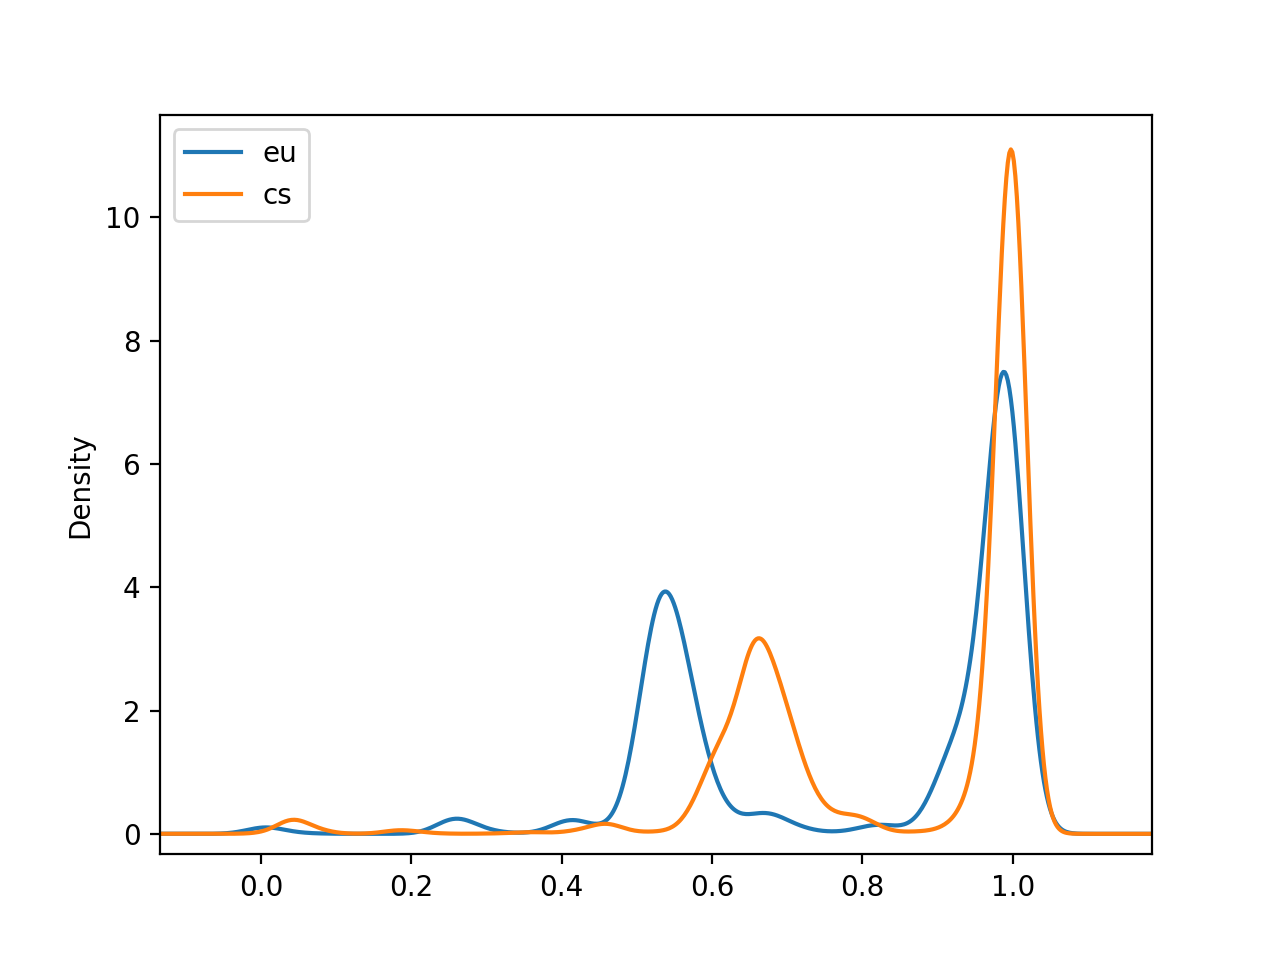
\includegraphics[width=.7\textwidth]{fig/metric_density.png}
\caption{Gaussian Kernel Density Estimate plot showing the distributions present for the \{0,1\} scaled euclidean and cosine distances.}
\label{fig:density2}
\end{figure}



A comparison of both similarities on the $x-y$ plot -  \autoref{fig:morig}. As many species have similar lifetimes, these are often situated within the same temporal space, which can make it hard to visually or interactively separate them. To overcome this, it is possible to convert the scatter plot into a force-simulation, \autoref{fig:metric}. Here nodes repulse each other and are attracted to their original location. This expands the graph and prevents overlapping nodes. In doing so it is possible to interactively query the pairs of nodes which are represented by each point if required. 




\begin{figure}[H]
\begin{subfigure}[t]{.5\textwidth}
  \centering
  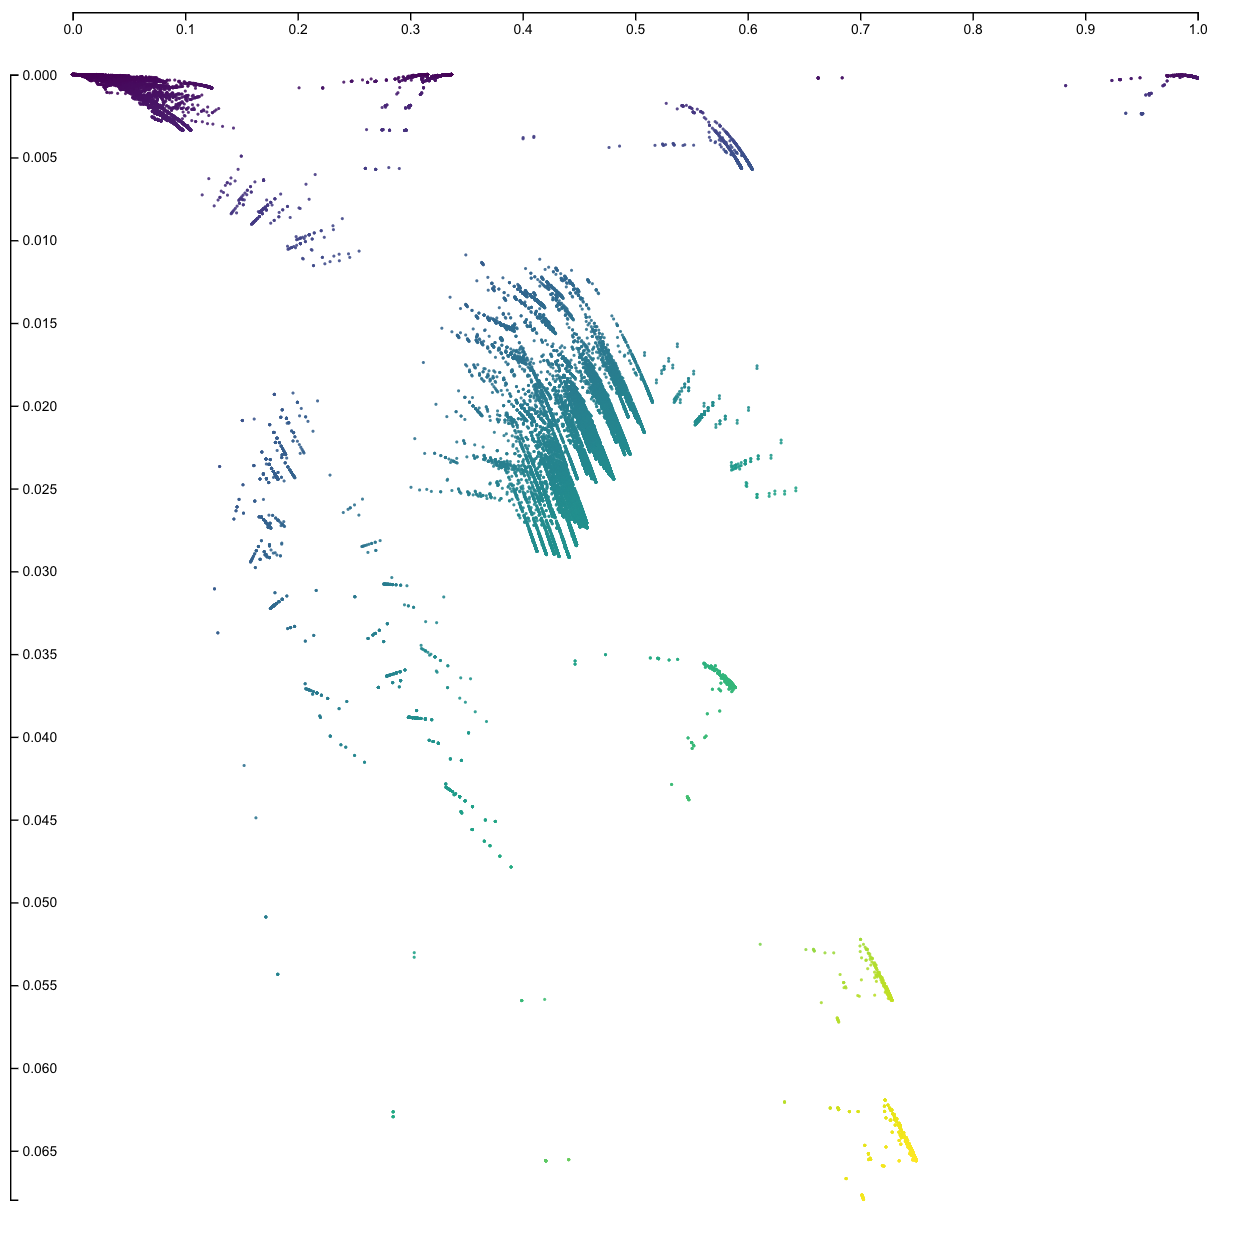
\includegraphics[width=\textwidth]{fig/metric-1.png}
  \caption{Original}
  \label{fig:morig}
\end{subfigure}%
\begin{subfigure}[t]{.5\textwidth}
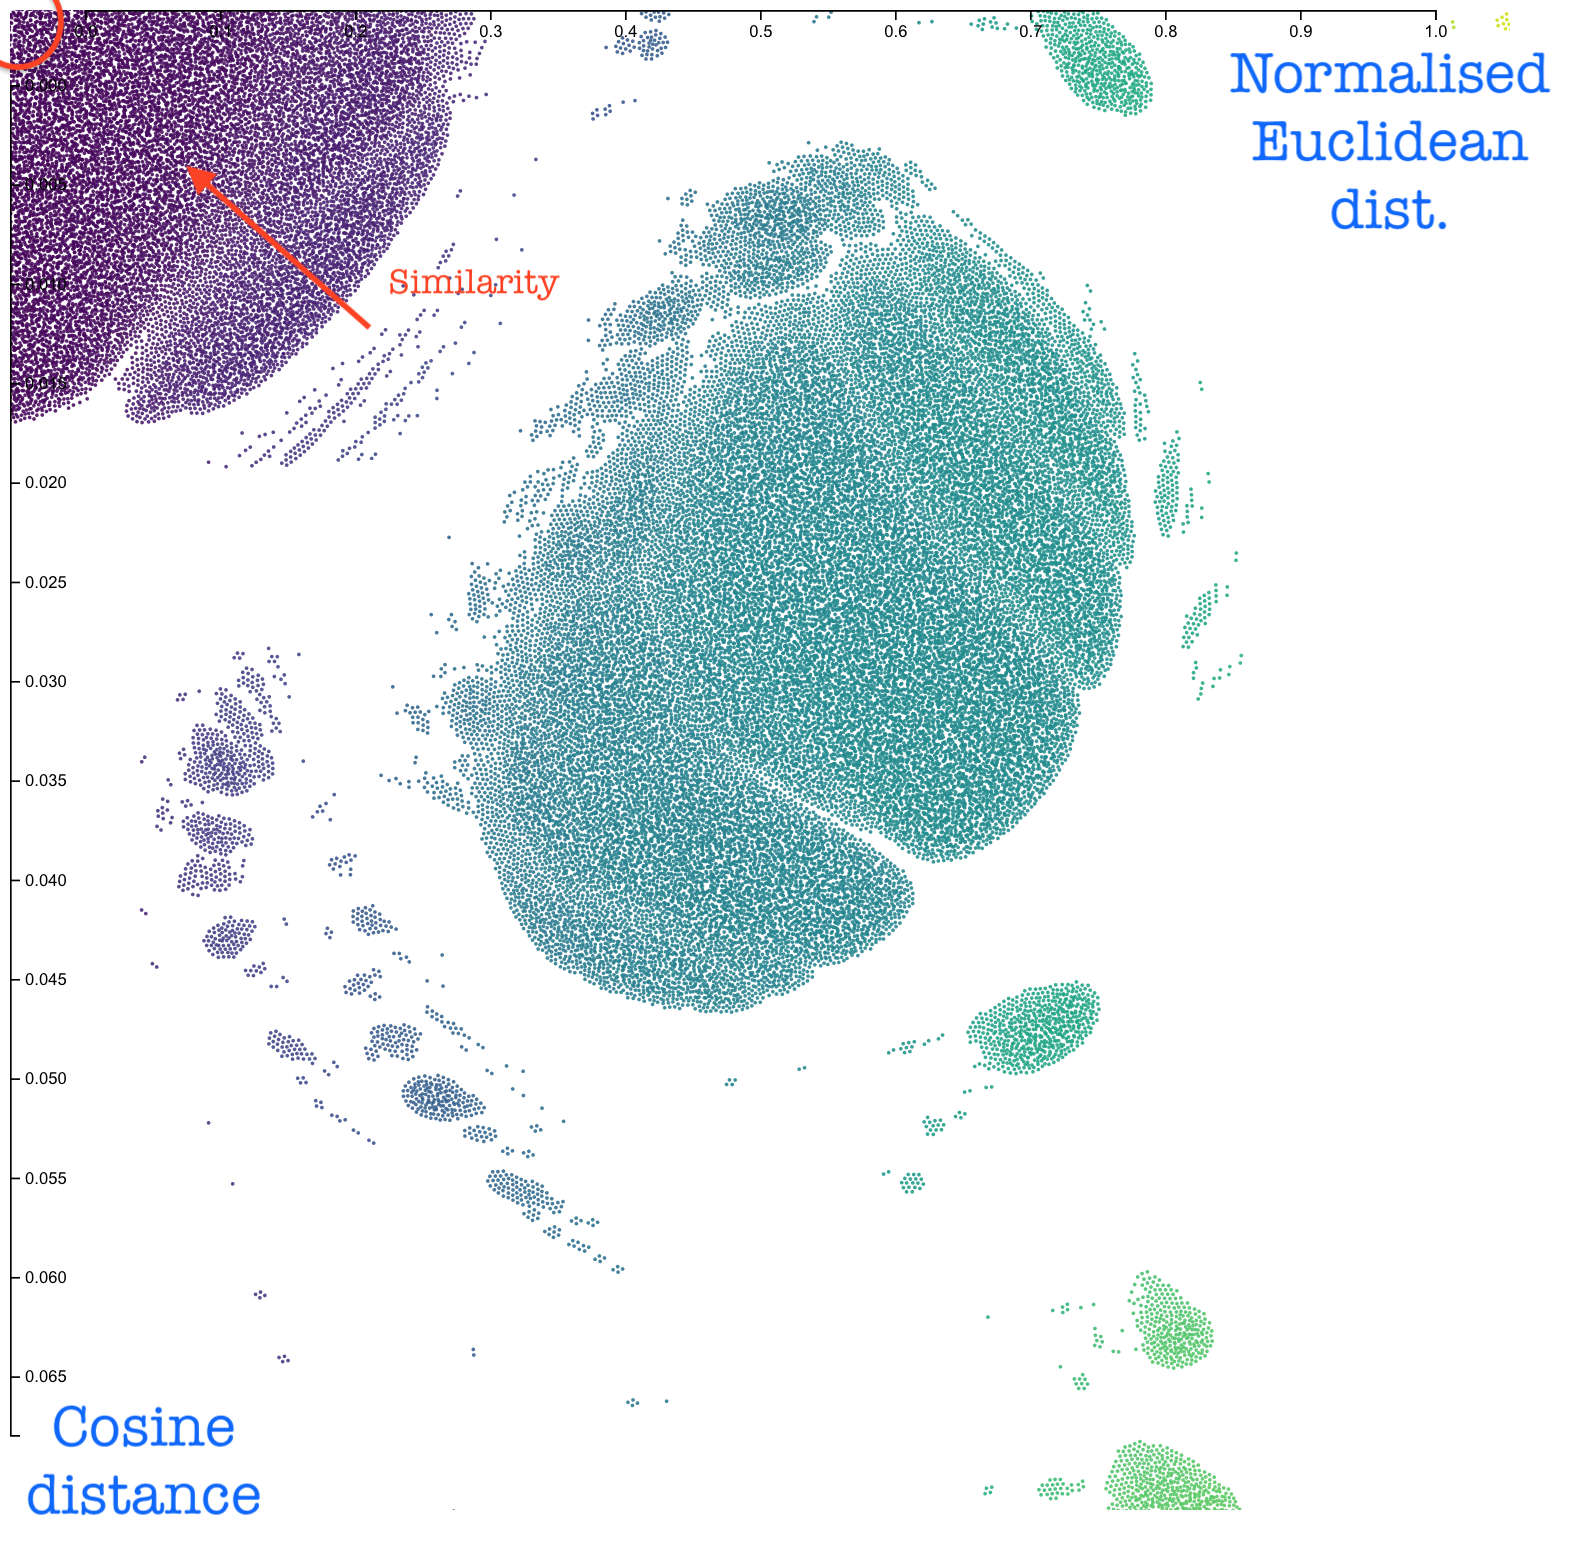
\includegraphics[width=\textwidth]{fig/metric.png}
\caption{No-overlap}
\label{fig:metric}
\end{subfigure}
\caption{Showing the evolution from the original overlaid locations, \autoref{fig:morig} to the slightly more accessible (interactively) \autoref{fig:metric}}
\end{figure}

Using a Kernel density plot it is seen that both cosine and euclidean distances have a similar distribution of points for the chosen simulation. The agreement of both metrics suggests a similarity between both the lifetime values and their change over time for simulation. This is in agreement of with the $x-y$ plot of the species. In selecting species that are part of the same initial cluster and have a high agreement between both similarities it is possible to gauge the suitability for two species to be lumped together. 


\subsection{A quick concnentration comparison}
Having described how the similarity distances work, the best and worst pairings are shown. The results in \autoref{fig:bestworst} - a log10 ensemble of the concentrations for the 300 sumulations used in the results section. Here the best matches both have a flat decay curve, whereas the the worst parings are between photolytically influenced species with a pronounced diurnal profile compared to ones with a flat loss curve.   


\begin{figure}[H]
\begin{subfigure}[t]{.5\textwidth}
  \centering
  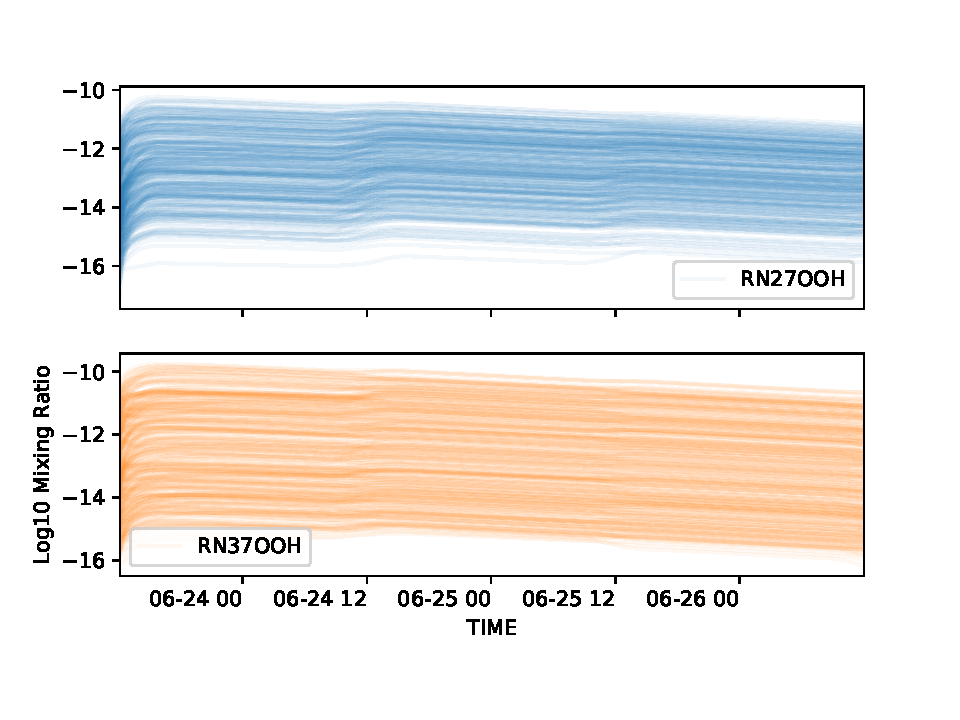
\includegraphics[width=\textwidth]{ensemble/RN27OOH-RN37OOH.pdf}
\end{subfigure}%
\begin{subfigure}[t]{.5\textwidth}
  \centering
  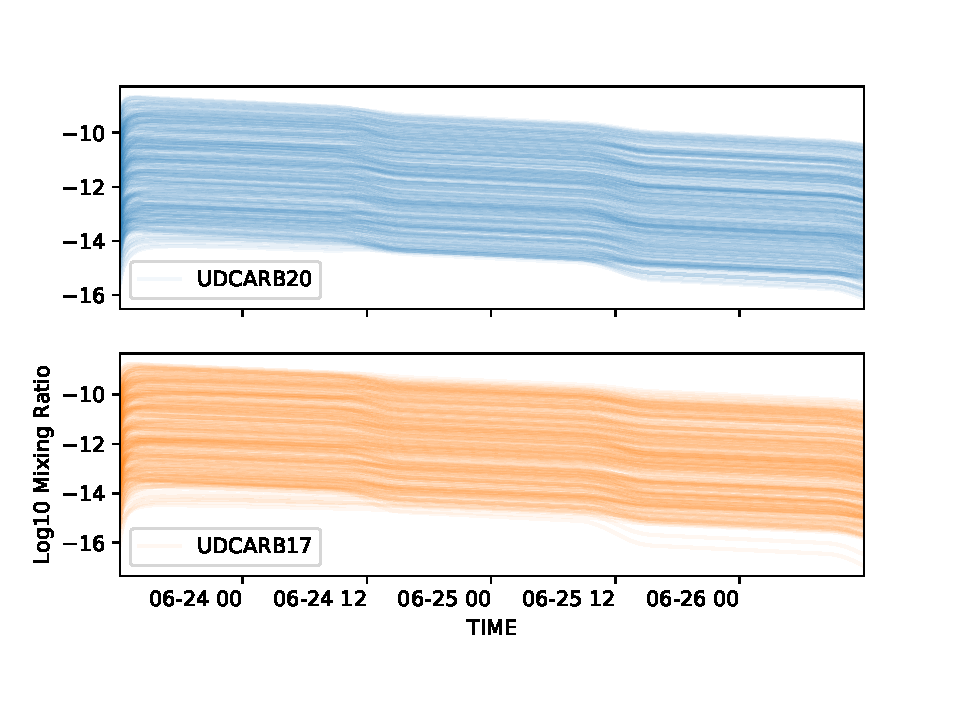
\includegraphics[width=\textwidth]{ensemble/UDCARB20-UDCARB17.pdf}
\end{subfigure}%\\

\begin{subfigure}[t]{.5\textwidth}
  \centering
  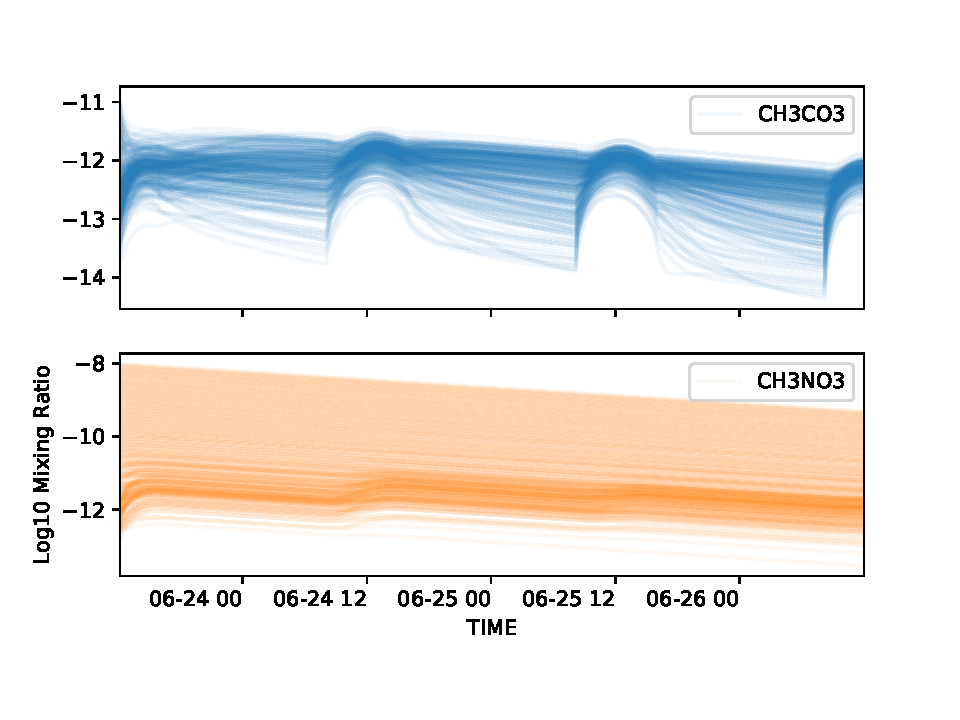
\includegraphics[width=\textwidth]{ensemble/CH3CO3-CH3NO3.pdf}
\end{subfigure}%
\begin{subfigure}[t]{.5\textwidth}
  \centering
  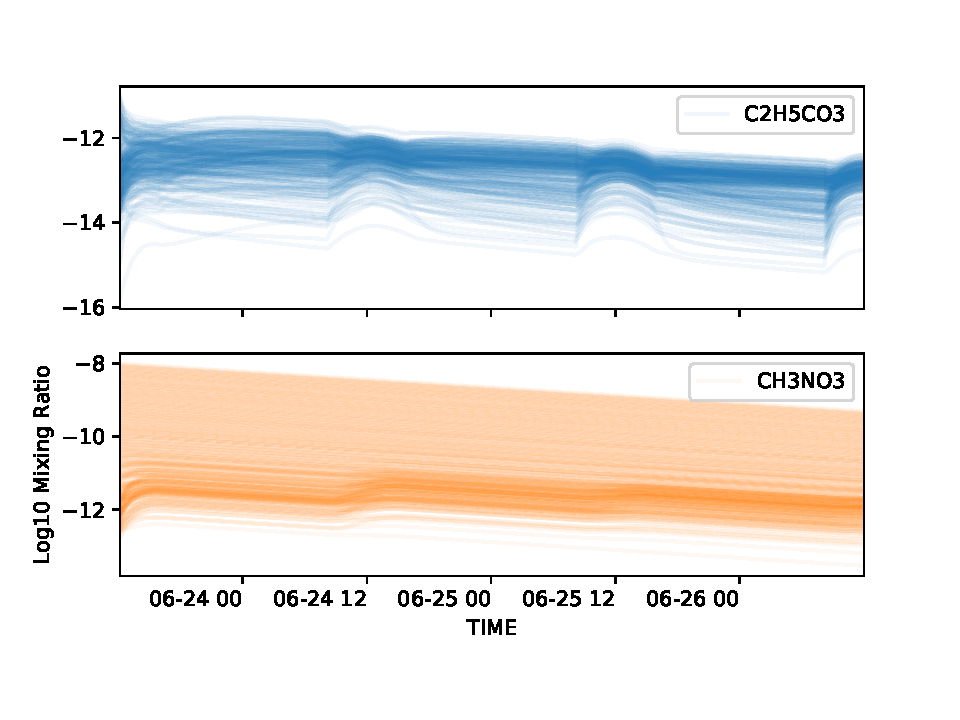
\includegraphics[width=\textwidth]{ensemble/C2H5CO3-CH3NO3.pdf}
\end{subfigure}%\\
\caption{\textbf{Comparing the best (a-b) and worst (c-d) species combinations using the combigned similarity metrics.} }
\label{fig:bestworst}
\end{figure}





